%%% Copyright (C) 2021  Luigi D. C. Soares
%%% 
%%% This program is free software: you can redistribute it and/or modify
%%% it under the terms of the GNU General Public License as published by
%%% the Free Software Foundation, either version 3 of the License, or
%%% (at your option) any later version.
%%% 
%%% This program is distributed in the hope that it will be useful,
%%% but WITHOUT ANY WARRANTY; without even the implied warranty of
%%% MERCHANTABILITY or FITNESS FOR A PARTICULAR PURPOSE.  See the
%%% GNU General Public License for more details.
%%% 
%%% You should have received a copy of the GNU General Public License
%%% along with this program.  If not, see <https://www.gnu.org/licenses/>.


%%%%%%%%%%%%%%%%%%%%%%%%%%%%%%%%%%%%%%%%%%%%%%%%%%%%%%%%%%%%%%%%
%%%%%%%%%%%%%%%%%%%%%%%% Beamer Options %%%%%%%%%%%%%%%%%%%%%%%%
%%%%%%%%%%%%%%%%%%%%%%%%%%%%%%%%%%%%%%%%%%%%%%%%%%%%%%%%%%%%%%%%
%%% t = frames default to top alignment
%%% Aspect ratio: 43 = 4:3, 169 = 16:9, ...
\documentclass[t, aspectratio=169]{beamer}

%%%%%%%%%%%%%%%%%%%%%%%%%%%%%%%%%%%%%%%%%%%%%%%%%%%%%%%%%%%%%%%%
%%%%%%%%%%%%%%%%%%%%%%%% Custom Settings %%%%%%%%%%%%%%%%%%%%%%%
%%%%%%%%%%%%%%%%%%%%%%%%%%%%%%%%%%%%%%%%%%%%%%%%%%%%%%%%%%%%%%%%
%%% Copyright (C) 2021  Luigi D. C. Soares
%%% 
%%% This program is free software: you can redistribute it and/or modify
%%% it under the terms of the GNU General Public License as published by
%%% the Free Software Foundation, either version 3 of the License, or
%%% (at your option) any later version.
%%% 
%%% This program is distributed in the hope that it will be useful,
%%% but WITHOUT ANY WARRANTY; without even the implied warranty of
%%% MERCHANTABILITY or FITNESS FOR A PARTICULAR PURPOSE.  See the
%%% GNU General Public License for more details.
%%% 
%%% You should have received a copy of the GNU General Public License
%%% along with this program.  If not, see <https://www.gnu.org/licenses/>.

%%%%%%%%%%%%%%%%%%%%%%%%%%%%%%%%%%%%%%%%%%%%%%%%%%%%%%%%%%%%%%%%
%%%%%%%%%%%%%%%%%%%%%%%%%%% Packages %%%%%%%%%%%%%%%%%%%%%%%%%%%
%%%%%%%%%%%%%%%%%%%%%%%%%%%%%%%%%%%%%%%%%%%%%%%%%%%%%%%%%%%%%%%%
\usepackage[utf8]{inputenc}
\usepackage[T1]{fontenc}
\usepackage{bm}
\usepackage{mathtools}
\usepackage{stmaryrd}
\usepackage{minted}
\usepackage{tikz}
\usepackage[style=authoryear, citestyle=authortitle]{biblatex}

%%%%%%%%%%%%%%%%%%%%%%%%%%%%%%%%%%%%%%%%%%%%%%%%%%%%%%%%%%%%%%%%
%%%%%%%%%%%%%%%%%%%%%%% Logo Positioning %%%%%%%%%%%%%%%%%%%%%%%
%%%%%%%%%%%%%%%%%%%%%%%%%%%%%%%%%%%%%%%%%%%%%%%%%%%%%%%%%%%%%%%%
\logo{\begin{tikzpicture}[overlay, remember picture]
    \node[left=0.2cm] at ([yshift=-1cm] current page.north east)
        {\includegraphics
        [width=.125\paperwidth, keepaspectratio]{logo.png}};
\end{tikzpicture}}

%%%%%%%%%%%%%%%%%%%%%%%%%%%%%%%%%%%%%%%%%%%%%%%%%%%%%%%%%%%%%%%%
%%%%%%%%%%%%%%%%%%%%%%%%% Other Settings %%%%%%%%%%%%%%%%%%%%%%%
%%%%%%%%%%%%%%%%%%%%%%%%%%%%%%%%%%%%%%%%%%%%%%%%%%%%%%%%%%%%%%%%
%%% By default, every numbered environment share the same
%%% counter as theorem. We can redefine them so that they
%%% have their own counter. Notice, however, that the Beamer
%%% user guide strongly discourages that, because this way
%%% there might be, for example, a Definition 2 after a
%%% Theorem 10, which (according to them) make things harder
%%% to find. Personally, I disagree; I find it weird to have,
%%% for instance, an Example 2 without an Example 1.
\undef{\example}
\theoremstyle{example}
\newtheorem{example}{Example}
%%% We can also disable numbering entirely:
% \setbeamertemplate{theorems}[default]

%%% Make math font look line in articles.
\usefonttheme[onlymath]{serif}

%%% Math operators.
\DeclareMathOperator{\Def}{\coloneqq}

\makeatletter
\newcommand{\To}{\@ifstar{\@ToB}{\@ToA}}
\newcommand{\@ToA}[1]{\xrightarrow{#1}}
\newcommand{\@ToB}[2]{%
  \xrightarrow{#1}\mathrel{\vphantom{\to}^{#2}}}
\makeatother

%%% Minted config.
\usemintedstyle{monokai}
\renewcommand\theFancyVerbLine{\arabic{FancyVerbLine}}
\setminted[idris]{
    fontfamily=courier,
    frame=lines,
    framesep=2mm,
    breaklines,
    linenos,
    numbersep=5pt,
    stripnl=false,
    autogobble,
    escapeinside=@@
}

%%% Tikz config.
%%% Libraries:
\usetikzlibrary{
    arrows.meta,
    decorations.pathmorphing,
    positioning,
    tikzmark}
%%% TikZ style to apply keys only on specific beamer overlays
%%% only=<overlay spec>{key=value, key=value, ...}
\tikzset{only/.code args={<#1>#2}{%
  \only<#1>{\pgfkeysalso{#2}}%
}}
%%% Default tikz origin coordinates to the center of the page.
%%% Use \shifttikz{<node>}{<shift x>}{<shift y>}{<tikz picture>}
%%% to shift the origin of a tikz picture. For this to work, your
%%% tikz picture must have the following option:
%%% shift = {([xshift = \tikzxshift, yshift = \tikzyshift] \tikzorigin)}
\newcommand{\tikzorigin}{current page.center}
\newlength{\tikzxshift}
\newlength{\tikzyshift}
\setlength{\tikzxshift}{0cm}
\setlength{\tikzyshift}{0cm}
\newcommand{\shifttikz}[4]{{%
    \renewcommand{\tikzorigin}{#1}%
    \setlength{\tikzxshift}{#2}%
    \setlength{\tikzyshift}{#3}%
    #4%
}}

%%% References file.
\addbibresource{references.bib}

%%%%%%%%%%%%%%%%%%%%%%%%%%%%%%%%%%%%%%%%%%%%%%%%%%%%%%%%%%%%%%%%
%%%%%%%%% Information to be included in the title page %%%%%%%%%
%%%%%%%%%%%%%%%%%%%%%%%%%%%%%%%%%%%%%%%%%%%%%%%%%%%%%%%%%%%%%%%%
\title[Secure Compilation]{%
    On the Secure Compilation of the Constant-Time 
    Policy}
\subtitle{Quantitative Information Flow}
\author[luigi.domenico@dcc.ufmg.br]{%
    Luigi D. C. Soares\texorpdfstring{\\}{}
    (\texttt{luigi.domenico@dcc.ufmg.br})}
\institute[DCC/UFMG]{%
    Department of Computer Science \\
    Federal University of Minas Gerais}
\date[2021/1]{}

\usetheme{saori}

\begin{document}

\begin{frame}
\titlepage
\end{frame}

\input{include/frames/side-channels}
%%% Copyright (C) 2021  Luigi D. C. Soares
%%% 
%%% This program is free software: you can redistribute it and/or modify
%%% it under the terms of the GNU General Public License as published by
%%% the Free Software Foundation, either version 3 of the License, or
%%% (at your option) any later version.
%%% 
%%% This program is distributed in the hope that it will be useful,
%%% but WITHOUT ANY WARRANTY; without even the implied warranty of
%%% MERCHANTABILITY or FITNESS FOR A PARTICULAR PURPOSE.  See the
%%% GNU General Public License for more details.
%%% 
%%% You should have received a copy of the GNU General Public License
%%% along with this program.  If not, see <https://www.gnu.org/licenses/>.

\begin{frame}{Defense Strategy}
\begin{definition}[Constant-Time Programming]<2->
    A program is said to implement a constant-time policy if
    \only<3->{its memory accesses}
    \only<4->{and control flow}
    \only<5->{do not depend on secret information.}
    \only<6->{In other words, the sequence of instructions
    and memory accesses must be the same regardless
    of the secret inputs.}
\end{definition}
\end{frame}
%%% Copyright (C) 2021  Luigi D. C. Soares
%%% 
%%% This program is free software: you can redistribute it and/or modify
%%% it under the terms of the GNU General Public License as published by
%%% the Free Software Foundation, either version 3 of the License, or
%%% (at your option) any later version.
%%% 
%%% This program is distributed in the hope that it will be useful,
%%% but WITHOUT ANY WARRANTY; without even the implied warranty of
%%% MERCHANTABILITY or FITNESS FOR A PARTICULAR PURPOSE.  See the
%%% GNU General Public License for more details.
%%% 
%%% You should have received a copy of the GNU General Public License
%%% along with this program.  If not, see <https://www.gnu.org/licenses/>.

\begin{frame}{Password Checker}
\stepcounter{beamerpauses}
\begin{example}<+->
    Consider the case of a $n$-bit password checker
    \only<+->{that either rejects the $i$-th bit or accepts the user's guess.}
    \only<+->{It could be implemented as follows:}
    \only<+->{\inputminted{idris}{include/code/check.idr}}
    \only<+->{%%% Copyright (C) 2021  Luigi D. C. Soares
%%% 
%%% This program is free software: you can redistribute it and/or modify
%%% it under the terms of the GNU General Public License as published by
%%% the Free Software Foundation, either version 3 of the License, or
%%% (at your option) any later version.
%%% 
%%% This program is distributed in the hope that it will be useful,
%%% but WITHOUT ANY WARRANTY; without even the implied warranty of
%%% MERCHANTABILITY or FITNESS FOR A PARTICULAR PURPOSE.  See the
%%% GNU General Public License for more details.
%%% 
%%% You should have received a copy of the GNU General Public License
%%% along with this program.  If not, see <https://www.gnu.org/licenses/>.

\begin{tikzpicture}[remember picture, overlay]
    \draw[fill=gray, fill opacity=0.1]
    ([shift={(-.5cm, .3cm)}] pic cs:sc:st) 
    rectangle 
    ([shift={(.25cm, -.15cm)}] pic cs:sc:end);
    
    \draw[Stealth-, decorate, decoration={snake,
        amplitude=.4mm, segment length=4.75mm, 
        pre length=1.75mm, post length=.25mm}
    ]
        ([shift={(.3cm, .25cm)}] pic cs:sc:end)
        --
        ([shift={(2.5cm, .25cm)}] pic cs:sc:end)
        node[right, align=left] {\tikzmark{sc-text:st}
            \large\emph{Side channel}\tikzmark{sc-text:end}};
            
    \draw[fill=gray, fill opacity=0.1]
        ([shift={(-0.05cm, .5cm)}] pic cs:sc-text:st)
        rectangle
        ([shift={(0.2cm, -.3cm)}] pic cs:sc-text:end);
\end{tikzpicture}}
\end{example}
\end{frame}

\begin{frame}{Password Checker}
\stepcounter{beamerpauses}
\begin{example}
    Consider, again, the case of a $n$-bit password checker.
    \only<+->{%
        But, this time it either rejects or accepts the
        entire guessed password.}
    \only<+->{It could be implemented as follows:}
    \only<+->{\inputminted{idris}{include/code/check-safe.idr}}
\end{example}
\end{frame}

\begin{frame}{Password Checker}
\inputminted{idris}{include/code/check-safe.idr}
\begin{itemize}
    \item<2-| alert@2> Function ctsel stands for
        constant-time selector
        
    \item<3-| alert@3> Corresponds to x86's cmov
    
    \item<4-| alert@4> LLVM's x86-cmov-converter pass
        replaces cmovs with branches
        
    \item<5-| alert@5> How to prove that the constant-time property
        is preserved?
\end{itemize}
\end{frame}
%%% Copyright (C) 2021  Luigi D. C. Soares
%%% 
%%% This program is free software: you can redistribute it and/or modify
%%% it under the terms of the GNU General Public License as published by
%%% the Free Software Foundation, either version 3 of the License, or
%%% (at your option) any later version.
%%% 
%%% This program is distributed in the hope that it will be useful,
%%% but WITHOUT ANY WARRANTY; without even the implied warranty of
%%% MERCHANTABILITY or FITNESS FOR A PARTICULAR PURPOSE.  See the
%%% GNU General Public License for more details.
%%% 
%%% You should have received a copy of the GNU General Public License
%%% along with this program.  If not, see <https://www.gnu.org/licenses/>.

\begin{frame}{Secure Compilation}
\begin{itemize}
    \item<2-| alert@2> \cite{BartheSecure}
    % \item<2-| alert@2> Secure Compilation of Side-Channel Countermeasures:
    % The Case of Cryptographic ``Constant-Time'' --
    % Gilles Barthe, Benjamin Grégoire, Vincent Laporte
    
    \item<3-| alert@3> Observational non-interference
    \item<4-| alert@4> Constant-time simulations
\end{itemize}
\end{frame}

\begin{frame}{Secure Compilation}
\begin{itemize}
    \item<2-| alert@2-3> A state is of the form 
    $\left\{c, \rho\right\}$,
    \only<3->{where $c$ is a command and $\rho$ is an environment}
    
    \item<4-| alert@4> A program $P$ is composed by a sequence of
    commands
    
    \item<5-| alert@5-> The semantics of $P$ is modelled by
    labelled transitions of the form \[a \To*{t}{n} a',\]
    \only<6->{%
        where $a$ and $a'$ are states, $t$ is the leakage
        and $n$ is the number of steps}
\end{itemize}
\end{frame}

\begin{frame}{Secure Compilation}
\begin{definition}[Observational Non-Interference]
    Let $P(\mathcal{I})$ be the set of initial states of a
    program $P$ that is given a set $\mathcal{I}$ of inputs,
    \only<2->{let $\mathcal{S}$ be the set of states,}
    \only<3->{$\mathcal{S}_f$ the set of final states and}
    \only<4->{$\mathcal{L}$ the set of leakage.}
    \only<5->{%
        Then, $P$ is obs. non-interfering w.r.t.
        a binary relation $\phi$ on states,}
    \only<6->{written $P \models \mathrm{ONI}(\phi),$}
    \only<7->{%
        iff for all $a, a' \in P(\mathcal{I})$,
        $b, b' \in \mathcal{S}$ and
        $t, t' \in \mathcal{L}$,}
    \only<8->{%
        \[
            a \To*{t}{n} b \land a' \To*{t'}{n} b' \land
            a \mathbin{\phi} a' \implies
            t = t' \land 
            (b \in \mathcal{S}_f \iff b' \in \mathcal{S}_f).
        \]}
\end{definition}
\end{frame}

\begin{frame}{Secure Compilation}
\begin{definition}[Lockstep Simulation]
    $\approx$ is a lockstep simulation w.r.t. source and
    target programs $S$ and $C = \llbracket S\rrbracket$ when
    \begin{enumerate}
        \item<only@2-> $\forall$ source step $a \to b$ and
        target state $\alpha$ such that
        $a \approx \alpha$,
        \only<only@3->{%
            $\exists$ a target step $\alpha \to \beta$ such
            that $b \approx \beta$}

        \item<only@3-> $\forall$ input parameter $i$,
        we have $S(i) \approx C(i)$
        
        \item<only@4-> $\forall$ source and target states
        $b$ and $\beta$ such that $b \approx \beta$,
        \only<5->{%
            we have that $b$ is a final source state iff
            $\beta$ is a final target state}
    \end{enumerate}
\end{definition}
\end{frame}

\begin{frame}{Secure Compilation}
%%% Copyright (C) 2021  Luigi D. C. Soares
%%% 
%%% This program is free software: you can redistribute it and/or modify
%%% it under the terms of the GNU General Public License as published by
%%% the Free Software Foundation, either version 3 of the License, or
%%% (at your option) any later version.
%%% 
%%% This program is distributed in the hope that it will be useful,
%%% but WITHOUT ANY WARRANTY; without even the implied warranty of
%%% MERCHANTABILITY or FITNESS FOR A PARTICULAR PURPOSE.  See the
%%% GNU General Public License for more details.
%%% 
%%% You should have received a copy of the GNU General Public License
%%% along with this program.  If not, see <https://www.gnu.org/licenses/>.

\begin{tikzpicture}[
    remember picture,
    overlay,
    shift = {([xshift = \tikzxshift, yshift = \tikzyshift] \tikzorigin)},
    font=\Large
]
    \node (a) at (-2cm, 2cm) {$a$};
    \node (b) at (2cm, 2cm)  {$b$};
    
    \node (alpha) at (-2cm, -2cm) {$\alpha$};
    
    \node [color = darkred!83] (beta) at (2cm, -2cm) {$\bm{\beta}$};
        
    \draw [-Latex, thick] (a) -- (b);
    
    \draw [-Latex, thick, color = darkred!83]
        (alpha) -- (beta);
        
    \draw [thick, dotted, shorten >= .1cm, shorten <= .1cm]
        (a) -- (alpha)
        node [midway, left] {$\approx$};
        
    \draw [
        thick, dotted, shorten >= .1cm,
        shorten <= .1cm, color = darkred!83
    ]   
        (b) -- (beta)
        node [midway, right, color = darkred!83] {$\bm{\approx}$};
\end{tikzpicture}
\end{frame}

\begin{frame}{Secure Compilation}
\begin{definition}[Lockstep CT-Simulation]
    $(\equiv_S, \equiv_C)$ is a lockstep CT-simulation w.r.t.
    $\approx$ iff:
    \begin{enumerate}
        \item<only@2-> $\forall$ source steps
        $a \To{t} b$ and $a' \To{t} b'$ such that
        $a \equiv_S a'$, and
        \only<3->{%
            $\forall$ target steps $\alpha \To{\tau} \beta$
            and $\alpha' \To{\tau'} \beta'$ such that
            $a \approx \alpha$, $a' \approx \alpha'$, 
            $\alpha \equiv_C \alpha'$, $b \approx \beta$
            and $b' \approx \beta'$}
        \only<4->{%
            it follows that $b \equiv_S b'$, $\beta \equiv_C \beta'$
            and $\tau = \tau'$}
            
        \item<only@5-> $\forall$ pairs of input parameters
        $i$ and $i'$ such that $i \mathbin{\varphi} i'$,
        \only<6->{we have that $S(i) \equiv_S S(i')$ and
        $C(i) \equiv_C C(i')$, where $\varphi$ is a binary
        relation on inputs}
    \end{enumerate}
\end{definition}
\end{frame}

\begin{frame}{Secure Compilation}
%%% Copyright (C) 2021  Luigi D. C. Soares
%%% 
%%% This program is free software: you can redistribute it and/or modify
%%% it under the terms of the GNU General Public License as published by
%%% the Free Software Foundation, either version 3 of the License, or
%%% (at your option) any later version.
%%% 
%%% This program is distributed in the hope that it will be useful,
%%% but WITHOUT ANY WARRANTY; without even the implied warranty of
%%% MERCHANTABILITY or FITNESS FOR A PARTICULAR PURPOSE.  See the
%%% GNU General Public License for more details.
%%% 
%%% You should have received a copy of the GNU General Public License
%%% along with this program.  If not, see <https://www.gnu.org/licenses/>.

\begin{tikzpicture}[
    remember picture,
    overlay,
    shift = {([xshift = \tikzxshift, yshift = \tikzyshift] \tikzorigin)},
    font=\Large,
    equivcolor/.store in = \equivcolor,
    equivcolor = white,
    equiv/.style = {
        color = \equivcolor,
        %%% Draw the extremities of the \equiv symbol: 
        %%% first draw a very thick line and then draw
        %%% another line with the background color; 
        preaction = {
            draw, line width = 3.8pt, color = \equivcolor,
            postaction = {
                draw,
                line width = 2.2pt, color = background,
                shorten >= -.1cm, shorten <= -.1cm
            }
        }
    }
]
    \node (a)  at (-3.25cm, 1.25cm) {$a$};
    \node (a') at (-2cm, 2.5cm)     {$a'$};
    \node (b)  at (0.75cm, 1.25cm)  {$b$};
    \node (b') at (2cm, 2.5cm)      {$b'$};
    
    \node (alpha)  at (-3.25cm,-2.75cm) {$\alpha$};
    \node (alpha') at (-2cm, -1.5cm)    {$\alpha'$};
    \node (beta)   at (0.75cm, -2.75cm) {$\beta$};
    \node (beta')  at (2cm, -1.5cm)   {$\beta'$};
    
    \draw [-Latex, thick] 
        (a) -- (b) node [midway, above] {$t$};    
    \draw [-Latex, thick] 
        (a') -- (b') node [midway, above] {$t$};
    
    \draw [-Latex, thick]
        (alpha) -- (beta)
        node [midway, above, color = darkred!83] {$\bm{\tau}$};
    \draw [-Latex, thick]
        (alpha') -- (beta')
        node [midway, above, color = darkred!83] {$\bm{\tau}$};
    
    \draw [thick, dotted, shorten >= .1cm, shorten <= .1cm]
        (a) -- (alpha)
        node [midway, left] {$\approx$};    
    \draw [thick, dotted, shorten >= .1cm, shorten <= .1cm]
        (a') -- (alpha')
        node [midway, left] {$\approx$};
    
    \draw [thick, dotted, shorten >= .1cm, shorten <= .1cm]
        (b) -- (beta)
        node [midway, right] {$\approx$};    
    \draw [thick, dotted, shorten >= .1cm, shorten <= .1cm]
        (b') -- (beta')
        node [midway, right] {$\approx$};
        
    \draw [thick, equiv] (a) -- (a');
    \draw [thick, equiv, equivcolor = darkred!83] (b) -- (b');
    \draw [thick, equiv] (alpha) -- (alpha');
    \draw [thick, equiv, equivcolor = darkred!83] (beta) -- (beta');
\end{tikzpicture}
\end{frame}

\begin{frame}{Secure Compilation}
\begin{itemize}
    \item<+-> Let $[e]_{\rho}$ be the value of expression $e$
    under environment $\rho$
    \item<+-> Let $a.\mathrm{cmd}$ and $a.\mathrm{env}$ be the
    components of state $a$
\end{itemize}

\begin{example}[Constant Folding]<+->
    Constant folding reduces expressions whose operands are known. For example:
    \begin{enumerate}
        \item<only@+-> $
            \left(\forall \rho : [e_1]_{\rho} = 0\right)
            \implies
            \llbracket x \Def e_1 * e_2\rrbracket = x \Def 0
        $
        
        \item<only@+-> $
            \left(\forall \rho : [e_1]_{\rho} = 1\right)
            \implies
            \llbracket x \Def e_1 * e_2\rrbracket = x \Def e_2
        $
    \end{enumerate}
    
    \only<+->{Thus, it suffices to define}
    \begin{enumerate}
        \item<only@+-> $\approx$ as
        $
            \llbracket a.\mathrm{cmd}\rrbracket = \alpha.\mathrm{cmd}
            \land
            a.\mathrm{env} = \alpha.\mathrm{env}
        $ and
        
        \item<only@+-> $\equiv_S$ and $\equiv_C$ as
        $
            a.\mathrm{cmd} = b.\mathrm{cmd}
        $
    \end{enumerate}
\end{example}
\end{frame}

\begin{frame}{Secure Compilation}
\stepcounter{beamerpauses}
\begin{columns}
    \begin{column}{.5\textwidth}
        \begin{itemize}
            \item<+-> Let $a.\mathrm{cmd}$ and $a'.\mathrm{cmd}$
            be $y \Def A[i] * k$
            
            \item<+-> Let $b.\mathrm{cmd}$ and $b'.\mathrm{cmd}$ 
            be $z \Def x + y$
            
            \item<+-> Suppose $k$ always evaluates to $0$
            
            \item<+-> Then $\alpha.\mathrm{cmd}$ $\alpha'.\mathrm{cmd}$ 
            are $y \Def 0$
            
            \item<+-> Similarly, $\beta.\mathrm{cmd}$ and 
            $\beta'.\mathrm{cmd}$ are $z \Def x$
            
            \item<+-> $
                t = t' \cdot \left(A, [i]_{\rho_a}\right)
            $ and
            $
                [i]_{\rho_{a}} = [i]_{\rho_{a'}}
            $
            
            \item<+-> What is the leakage $\tau$ and is it the same
            in both steps?
            
            \item<+-> $\tau = \tau'$
        \end{itemize}
    \end{column}
    \begin{column}{.5\textwidth}
        \shifttikz{current page.east}{-.5\textwidth}{0cm}
            {%%% Copyright (C) 2021  Luigi D. C. Soares
%%% 
%%% This program is free software: you can redistribute it and/or modify
%%% it under the terms of the GNU General Public License as published by
%%% the Free Software Foundation, either version 3 of the License, or
%%% (at your option) any later version.
%%% 
%%% This program is distributed in the hope that it will be useful,
%%% but WITHOUT ANY WARRANTY; without even the implied warranty of
%%% MERCHANTABILITY or FITNESS FOR A PARTICULAR PURPOSE.  See the
%%% GNU General Public License for more details.
%%% 
%%% You should have received a copy of the GNU General Public License
%%% along with this program.  If not, see <https://www.gnu.org/licenses/>.

\begin{tikzpicture}[
    remember picture,
    overlay,
    shift = {([xshift = \tikzxshift, yshift = \tikzyshift] \tikzorigin)},
    font=\Large,
    equivcolor/.store in = \equivcolor,
    equivcolor = white,
    equiv/.style = {
        color = \equivcolor,
        %%% Draw the extremities of the \equiv symbol: 
        %%% first draw a very thick line and then draw
        %%% another line with the background color; 
        preaction = {
            draw, line width = 3.8pt, color = \equivcolor,
            postaction = {
                draw,
                line width = 2.2pt, color = background,
                shorten >= -.1cm, shorten <= -.1cm
            }
        }
    }
]
    \node (a)  at (-3.25cm, 1.25cm) {$a$};
    \node (a') at (-2cm, 2.5cm)     {$a'$};
    \node (b)  at (0.75cm, 1.25cm)  {$b$};
    \node (b') at (2cm, 2.5cm)      {$b'$};
    
    \node (alpha)  at (-3.25cm,-2.75cm) {$\alpha$};
    \node (alpha') at (-2cm, -1.5cm)    {$\alpha'$};
    \node (beta)   at (0.75cm, -2.75cm) {$\beta$};
    \node (beta')  at (2cm, -1.5cm)   {$\beta'$};
    
    \draw [-Latex, thick] 
        (a) -- (b) node [midway, above] {$t$};    
    \draw [-Latex, thick] 
        (a') -- (b') node [midway, above] {$t$};
    
    \draw [-Latex, thick]
        (alpha) -- (beta)
        node [midway, above, color = darkred!83] {$\bm{\tau}$};
    \draw [-Latex, thick]
        (alpha') -- (beta')
        node [midway, above, color = darkred!83] {$\bm{\tau}$};
    
    \draw [thick, dotted, shorten >= .1cm, shorten <= .1cm]
        (a) -- (alpha)
        node [midway, left] {$\approx$};    
    \draw [thick, dotted, shorten >= .1cm, shorten <= .1cm]
        (a') -- (alpha')
        node [midway, left] {$\approx$};
    
    \draw [thick, dotted, shorten >= .1cm, shorten <= .1cm]
        (b) -- (beta)
        node [midway, right] {$\approx$};    
    \draw [thick, dotted, shorten >= .1cm, shorten <= .1cm]
        (b') -- (beta')
        node [midway, right] {$\approx$};
        
    \draw [thick, equiv] (a) -- (a');
    \draw [thick, equiv, equivcolor = darkred!83] (b) -- (b');
    \draw [thick, equiv] (alpha) -- (alpha');
    \draw [thick, equiv, equivcolor = darkred!83] (beta) -- (beta');
\end{tikzpicture}}
    \end{column}
\end{columns}
\end{frame}
%%% Copyright (C) 2021  Luigi D. C. Soares
%%% 
%%% This program is free software: you can redistribute it and/or modify
%%% it under the terms of the GNU General Public License as published by
%%% the Free Software Foundation, either version 3 of the License, or
%%% (at your option) any later version.
%%% 
%%% This program is distributed in the hope that it will be useful,
%%% but WITHOUT ANY WARRANTY; without even the implied warranty of
%%% MERCHANTABILITY or FITNESS FOR A PARTICULAR PURPOSE.  See the
%%% GNU General Public License for more details.
%%% 
%%% You should have received a copy of the GNU General Public License
%%% along with this program.  If not, see <https://www.gnu.org/licenses/>.

\begin{frame}{Relation to QIF}
\stepcounter{beamerpauses}
\begin{columns}
    \begin{column}{.5\textwidth}
        \begin{itemize}
            \item<+-| alert@+> Labelled transitions
            \item<+-| alert@+> Leakage as a trace of events
            \item<+-| alert@+> Constant-time simulation
        \end{itemize}
    \end{column}
    \addtocounter{beamerpauses}{-3}
    \begin{column}{.5\textwidth}
        \begin{itemize}
            \item<+-| alert@+> Information-theoretic channels
            \item<+-| alert@+> Leakage as a real number
            \item<+-| alert@+> Refinement
        \end{itemize}
    \end{column}
\end{columns}
\end{frame}
\input{include/frames/references}

\end{document}